\headerbox{Likelihood Active Learning}{name=lal,span=2,column=1,row=0, below=bus,above=bottom}{

%The Bayesian inverse problem rewritten into BuS framework can be solved exploiting Subset Simulation (SuS) \cite{}, which is suitable for the estimation of the probability of rare events, such as the failure probability $\mathbb{P}_f$. %By setting $c^{-1} = \max_{\vec{x} \in \Dx} \Lk(\vec{x})$, the failure probability $\mathbb{P}_f$ can be extremely small
%In real applications, the computation of likelihood function evaluation can take minutes or even hours, it's then fundamental to limit the number of likelihood calls.
%Active Learning Reliability (ARL) \cite{arl, bbus} is a framework exploiting surrogate model techniques and uncertainty quantification which allows to gain information around the limit state surface (in BuS, $h(p, \vec{x}) \approx 0$) while limiting at the same time the number of forward model evaluations.
%More specifically, a Polynomial Chaos Kriging (PCK) \cite{pck}  surrogate is adopted for the log-likelihood function and SuS is used to computationally solve the Bayesian inverse problem. 

\begin{multicols}{2}

\par\noindent
Starting from a set of initial training points, also called \textit{Experimental Design} (ED):
\begin{itemize}
\item $\mathcal{X} = \{\vec{x}^{(1)}, \dots, \vec{x}^{(N_0)}\} \subset \Dx$ 
\item $L = \{\Lk(\vec{x}^{(1)}), \dots, \Lk(\vec{x}^{(N_0)})\} \subset \R$
\end{itemize}
Likelihood Active Learning enriches $\mathcal{X}$ and $L$ in high probability zones. 

\par\noindent
The basic iterative procedure is composed of the following steps: 

\begin{enumerate}
\item Construct surrogate PCK $\hat{\ell}$ of $\log(\Lk)$ using current $\mathcal{X}$ and $L$.
\item Retrieve samples $\{(p_k,\vec{x}_k)\}_{k=1}^K$ distributed according to the subset $F_r$ of SuS using the surrogate limit state function
{\small $$ h_\ell(p,\vec{x}) = \log(p) - \log(c) - \hat{\ell}(\vec{x})$$}
\item Evaluate learning function and find best candidate for enrichment:
{\small $$\vec{x}^* = \argmin\limits_{k = 1,\dots,K} \frac{|\E[h_\ell(p_k, \vec{x}_k)]|}{\sqrt{\text{var}[h_\ell(p_k, \vec{x}_k)]}}$$}
\item Append $\vec{x}^*$ to $\mathcal{X}$ and $\Lk(\vec{x}^*)$ to $L$ and repeat from 1. until the target size ($> N_0$) is reached.
\end{enumerate} 

\columnbreak

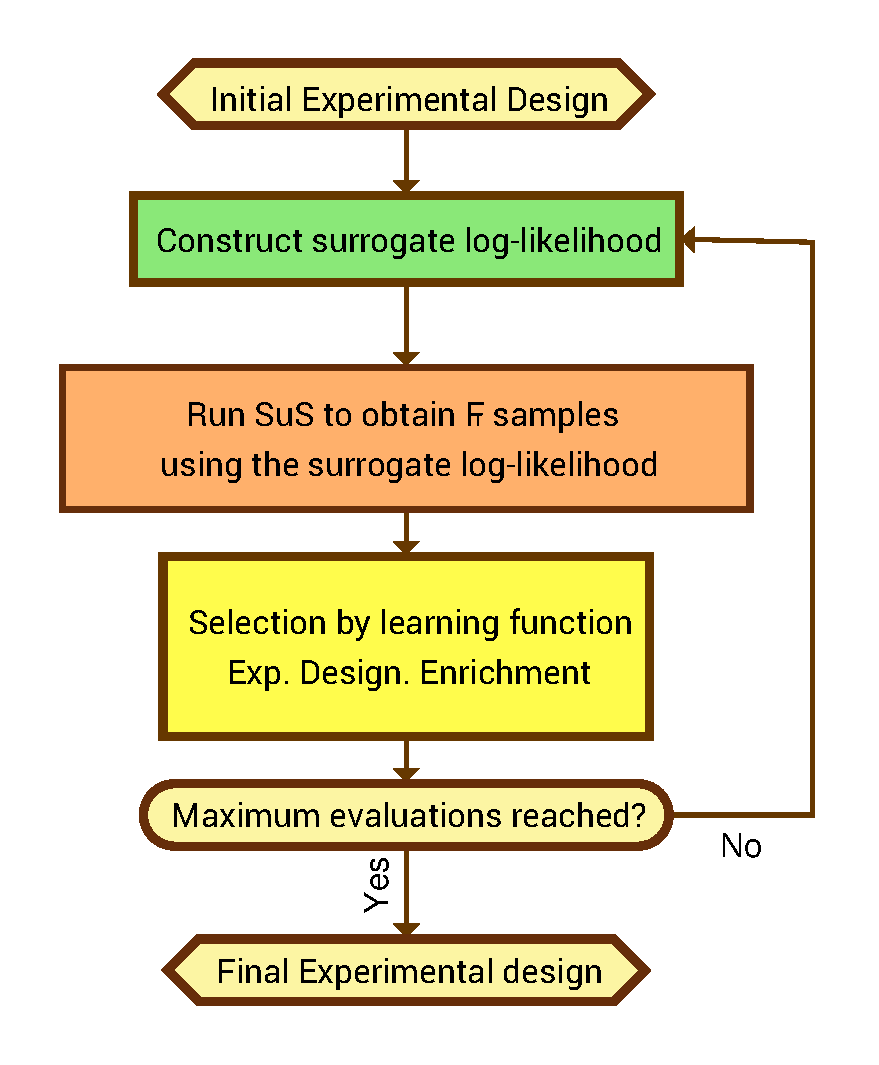
\includegraphics[width=0.5\textwidth]{schema_transparent.pdf}
\end{multicols}

\begin{minipage}{\textwidth}
    \centering
    \begin{minipage}{0.48\textwidth}
    \centering
        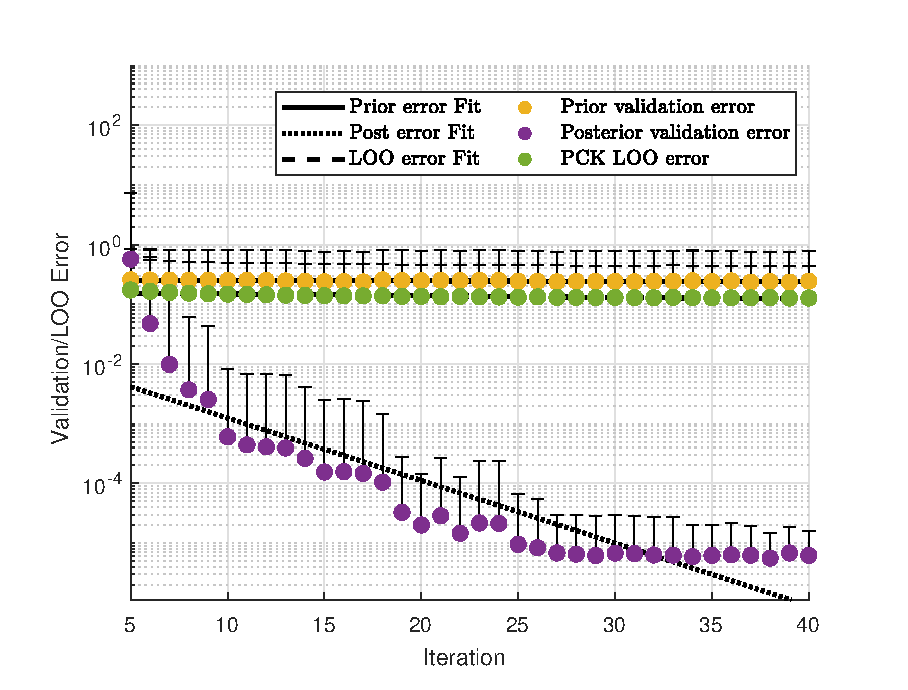
\includegraphics[width=0.9\textwidth]{validation_stat.eps}
        \captionof*{figure}{Validation error for the two-peaked test case along Likelihood Active Learning iterations.}
        %for the two-peaked Gaussian mixture case.}
    \end{minipage}
    \hspace{0.1cm}
    \begin{minipage}{0.48\textwidth}
        \centering
        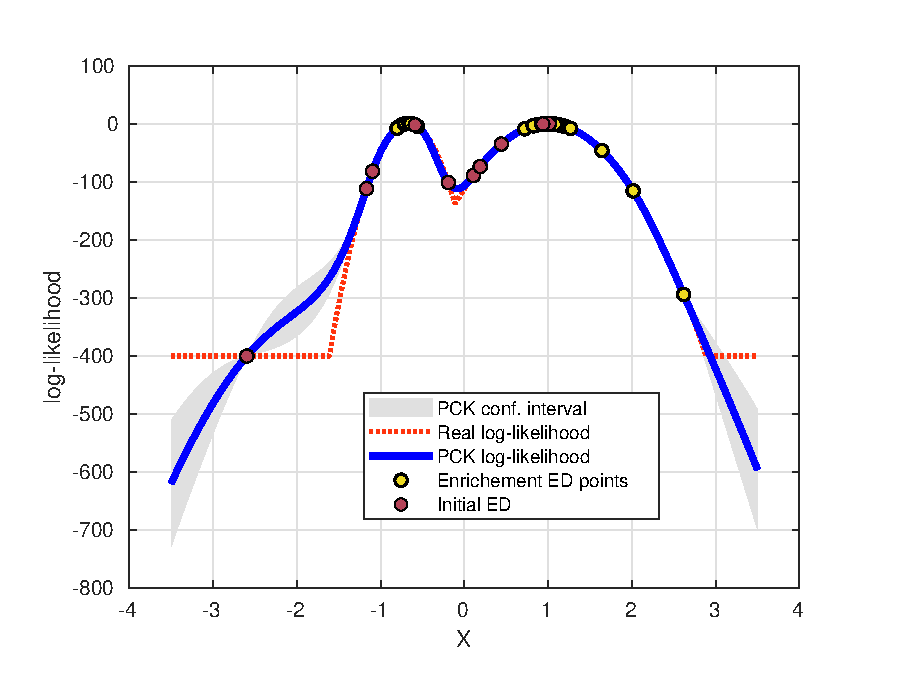
\includegraphics[width=0.9\textwidth]{kriging.eps}
        \captionof*{figure}{PCK visualization of Likelihood Active Learning enrichment for a two-peaked likelihood test case.}
    \end{minipage}
\end{minipage}

}

